\chapter{Particle Physics}
\section{Coassification of Elementary Particles}
\subsection{Leptons}
These are simplest and elementary particle with no internal structure known. They are  affected by electromagnetic, weak and gravitational forces but not by strong interaction.\\
These are three pairs:\\
Electrons $(e), \operatorname{Muon}(\mu), \operatorname{Tauon}(\tau)$, Electron-neutrino $\left(v_e\right)$, Muon-neutrino $\left(v_\mu\right)$,
Tau-neutrino $\left(v_r\right)$.\\
They also have corresponding antiparticles.
\subsection{Baryons}
Protons and particles heavier than proton form this group. Proton $(p)$ and neutron $(n)$ are called nucleons and rests are called Hyperons.\\
$\text { Hyperons }$ are a special class of baryons characterized by a time decay of the order of $\approx 10^{-10} \mathrm{sec}$ and mass value intermediate between those of the neutrons and deuteron. Their decay time is very much greater than the time of their formation time $\left(\approx 10^{-23} \mathrm{sec}\right)$.\\\\
It is because of this unsolved problem that these particles along with $K$-mesons are called strange particles.\\
Hyperons are $\operatorname{Lambda}(\Lambda), \operatorname{Sigma}\left(\Sigma^{\pm, 0}\right), \mathrm{Xi}\left(\Xi^0, \Xi^{-}\right)$, and $\operatorname{Omega}\left(\Omega^{-}\right)$.
\subsection{Mesons}
The rest mass of these particles varies between about $250 m_e$ to $1000 m_e$. They are the agent of interaction between the particles inside the nucleus. Mesons are Pions $\left(\pi^{+}, \pi^0, \pi^{-}\right)$, Kaons $\left(K^{+}, K^0\right)$ and $\operatorname{Eta}\left(\eta^0\right)$\\
Baryons and Mesons are together called as Hadrons.
\section{Particles and Anti-Particles}
The anti particle of a particle has the same mass, spin and lifetime if unstable, but its charge (if any) has the opposite sign. Thus the alignment between its spin and magnetic moment is also opposite to that of the particle.\\
\subsubsection{ (a) Electron and Positron}
Anti protons are produced by bombardment of $6 \mathrm{GeV}$ Protons
$$
p+p+(\text { energy }) \rightarrow p+p+p+\bar{p}
$$
The K.E. of bombarding proton is converted to a $p \& \bar{p}$ pair $+\mathrm{K}$. E of four particles.
Antiprotons interact strongly with matter \& annihilate with proton. In a typical annihilation reaction the rest mass of the annihilation pair appears as five pions and their K.E.
$$
p+\bar{p} \rightarrow \pi^{+}+\pi^{-}+\pi^{+}+\pi^{-}+\pi^0
$$
\subsubsection{ (c) Neutron and Anti-neutron}
The nature of anti-neutron is not well known. Both neutron and anti-neutron have zero charge and same mass. Since meutron is supposed to have certain internal chatge distribution it is expected that antineutrons has an opposite internal charge.\\
Anti-neutron is quickly annihilated either by a $p$ or $n$ usually with the production of several pions. \\
If anti-neutron is not annihilated by nucleons, then it decays by the reaction
$$
\bar{n} \rightarrow \bar{p}+e^{+}+v_e
$$
\subsubsection{ (d) Neutrino and Anti-neutrino}
Neutrino is elementary particle that has zero charge, $\frac{1}{2}$ spin, zero rest mass and nearly zero magnetic moment. It has finite energy and momentum in flight. It travel with speed of light $c$ and doesn't cause any ionization on passing through matter.\\
The anit-particle of neutrino is a anti-neutrino. The difference between neutrino and antineutrino is only in the sense of their helicity $(H)$.\\
The spin of neutrino $(v)$ is opposite in direction to the direction of its motion; viewed from behind, the neutrino spins counterclockwise. Neutrino moves in space in the manner of a lefthanded screw. Thus a neutrino possesses a "Left handed" helicity or negative helicity. The spin of anti-neutrino $(\bar{v})$ is in the same direction as its direction of motion; viewed from behind, the anti-neutrino spins clockwise. Neutrino moves in space in the manner of a righthanded screw. Thus a neutrino possesses a "Right handed" helicity or positive helicity.
\section{Elementary Particles Quantum Numbers}
\subsubsection{(a) Charge}
The elementary charges are 0 and $\pm e$.
\subsubsection{(b) Spin}
The spin quantum number is either an integer or an half odd integer for the particles so for detected\\
Bosons: spin $=0,1,2 \ldots$.\\ 
Fremions: spin $=1 / 2,3 / 2, \ldots \ldots$
\subsubsection{(c) Baryon Number (B)}
$+1$ assigned to all Baryons, $-1$ assigned to all anti-Baryons, 0 for others.
\subsubsection{(d) Lepton Number $\left(L_e, L_\mu, L_\tau\right)$}
\begin{align*}
L_e&=+1 \quad(\text { for electrons and } e \text {-neutrino) } \\
L_\mu&=+1 \quad(\text { for muon and } \mu \text {-neutrino) } \\
L_\tau&=+1 \quad \text { (for tauon and } \tau \text {-neutrino) }\\
\text{$-1$ is }&\text{assigned for their corresponding anti-particles and 0 is assigned for others.}
\end{align*}
\subsubsection{Stangeness Number (S)}
$\begin{array}{ll}
	S=+1 & \text { (for Kaons) } \\
	S=-1 & \text { (for } \Sigma \text {-Hyperons) }\\
	S=-1 & \text { (for } \Lambda \text {-Hyperons) } \\
	S=-2 & \text { (for } \Xi \text {-Hyperons) } \\
	S=-3 & \text { (for } \Omega \text {-Hyperons) }
\end{array}$
\subsubsection{Hypercharge (Y)}
Hypercharge is equal to the sum of strangeness and Baryon number of the particles families
$$
Y=B+S
$$
\subsubsection{(g) Isospin and Isotopic Quantum Number}
A number of hadrons families have members having similar masses but different charges. These families are called "multiplets" and multiplicity of these families are given by $2 I+1$, where $I$ is called the "Isotopic quantum number"\\
Ex: $\left(\pi^{+}, \pi^0, \pi^{-}\right) ;$Multiplicity $=2 I+1=3 \Rightarrow I=1$ ( for pions)\\
The components of isospin $I$ in an abstract "Isospace" in any specified direction is governed by a quantum number denoted by $I_3$. The possible values of $I_3$ are restricted to
\begin{align*}
&I,(I-1), \ldots \ldots \ldots, 0, \ldots \ldots \ldots-(I-1),-I\hspace{3cm}\text { ( } I \text { : integral) } \\
&I,(I-1), \ldots \ldots \ldots,-1 / 2,+1 / 2, \ldots \ldots \ldots-(I-1),-I\hspace{1.3cm}\text { ( } I \text { : half integral) }
\end{align*}
Ex: $\pi^{+} ; I_3=+1, \pi^0 ; I_3=0, \pi^{-} ; I_3=-1$\\\\
\renewcommand*{\arraystretch}{1.5}
\begin{tabular}{|c|c|c|c|c|c|c|c|c|c|c|c|}
	\hline
	Class & Name & Symbol & Spin & $B$ & $L_e$ & $L_\mu$ & $L_r$ & $S$ & $Y$ & $I$ & $I_3$	\\\hline
	\multirow{6}{*}{LEPTON}&Electron & $e^{-}$ & $\frac{1}{2}$ & 0 & $+1$ & 0 & 0&\multicolumn{4}{c|}{ }\\\cline{2-8}
	&Muon & $\mu^{-}$ & $\frac{1}{2}$ & 0 & 0 & $+1$ & 0 &\multicolumn{4}{c|}{ }\\\cline{2-8}
	 &Tauon & $\tau^{-}$ & $\frac{1}{2}$ & 0 & 0 & 0 & $+1$ &\multicolumn{4}{c|}{ }\\\cline{2-8}
	&$e$-neutrino & $v_e$ & $\frac{1}{2}$ & 0 & $+1$ & 0 & 0 &\multicolumn{4}{c|}{ }\\\cline{2-8}
	&$\mu$-neutrino & $v_{\mu }$ & $\frac{1}{2}$ & 0 & 0 & $+1$ & 0 &\multicolumn{4}{c|}{ }\\\cline{2-8}
	&$\tau$-neutrino & $v_r$ & $\frac{1}{2}$ & 0 & 0 & 0 & $+1$ &\multicolumn{4}{c|}{ }\\\hline
	\multirow{3}{*}{MESON}&Pion & $\pi^{\pm}, \pi^0$ & 0 & 0 & 0 & 0 & 0 & 0 & 0 & 1 & $\pm 1,0$ \\\cline{2-12}
	 &Kaon & $K^{+}, K^0$ & 0 & 0 & 0 & 0 & 0 & $+1$ & $+1$ & $\frac{1}{2}$ & $+\frac{1}{2},-\frac{1}{2}$ \\\cline{2-12}
	&$\eta$-meson & $\eta^0$ & 0 & 0 & 0 & 0 & 0 & 0 & 0 & 0 & 0 \\\hline
	\multirow{6}{*}{BAYRON}&Proton&$p$&\multirow{2}{*}{$\frac{1}{2}$}&\multirow{2}{*}{$+1$}& \multirow{2}{*}{0}&\multirow{2}{*}{0}&\multirow{2}{*}{0}&\multirow{2}{*}{0}&\multirow{2}{*}{$+1$}&\multirow{2}{*}{$\frac{1}{2}$} &        $+\frac{1}{2}$\\\cline{2-3}\cline{12-12}
	&Neutron&$n$& & & & & & & & &$-\frac{1}{2}$\\\cline{2-12}
	&$\Sigma$ Hyperon & $\Sigma^{\pm, 0}$ & $\frac{1}{2}$ & $+1$ & 0 & 0 & 0 & $-1$ & 0 & 1 & $\pm 1,0$ \\
	\cline{2-12}&$\Xi$ Hyperon & $\Xi^0, \Xi^{-}$ & $\frac{1}{2}$ & $+1$ & 0 & 0 & 0 & $-2$ & $-1$ & $\frac{1}{2}$ & $+\frac{1}{2},-\frac{1}{2}$ \\
	\cline{2-12}&$\Omega$ Hyperon & $\Omega^{-}$ & $\frac{3}{2}$ & $+1$ & 0 & 0 & 0 & $-3$ & $-2$ & 0 & 0 \\
	\cline{2-12}&$\Lambda$ Hyperon & $\Lambda^0$ & $\frac{1}{2}$ & $+1$ & 0 & 0 & 0 & $-1$ & 0 & 0 & 0\\\hline
\end{tabular}
\section{Classification of Fundamental Forces}
Four Basic interactions are summarized below:\\


	\begin{table}[H]
	\centering
	\renewcommand*{\arraystretch}{1.7}
	\begin{tabular}{|p{2.5cm}| p{1.5cm}|p{2cm}|p{2cm}|p{1.8cm}|}
			\hline Interaction & Particles Affected & Range & Relative Strength& Particle Exchanged \\
			\hline Strong & Hadrons & $\sim 10^{-15} \mathrm{~m}$ & 1 & Meson (Spin$=0$)\\\hline
			Electromagnetic&Charged Particles &$\infty$&$\sim 10^{-2}$&Photons (Spin$=1$)\\\hline
			Weak&Hadrons and Leptons &$\sim 10^{-17}m$&$\sim 10^{-13}$&Intermediate Bosons (Spin $=1$)\\\hline
			Gravitational&All&$\infty$&$\sim 10^{-40}$&Gravitons (Spin$=2$)\\\hline
	\end{tabular}
\end{table}


























\subsubsection{Quantum numbers that are conserved in all interactions}
\begin{enumerate}[label=\alph*)]
	\item  Charge
	\item  Spin
	\item  Baryon Number (B)
	\item  Lepton Number $\left(L_e, L_\mu, L_\tau\right)$
\end{enumerate}
\subsubsection{Quantum numbers that are conserved in some interactions}
Strong interactions:\hspace{3cm}$\Delta S=0, \Delta I=0, \Delta I_3=0$\\
Electromagnetic interactions:\hspace{1.3cm} $\Delta S=0, \Delta I \neq 0, \Delta I_3=0$\\
Weak interactions:\hspace{3.1cm}$\Delta S \neq 0, \Delta I \neq 0, \Delta I_3 \neq 0$
\begin{note}
	1. In weak interactions leptons are affected.\\
	2. In electromagnetic interactions photons are affected.\\
	3. In strong interactions mesons are affected.\\
\end{note}
\begin{exercise}
Identify the interactions if allowed\\
	(a) $\pi^{-}+p \rightarrow \Sigma^0+K^0$\hspace{2cm}
	(b) $\pi^{-}+p \rightarrow \pi^0+n$\\
	(c) $p+\gamma \rightarrow \pi^0+p$\hspace{2.5cm}
	(d) $\Sigma^0 \rightarrow \Lambda^0+\gamma$\\
	(e) $\pi^0 \rightarrow \gamma+\gamma$\hspace{3.2cm}
	(f) $K^0 \rightarrow \pi^{+}+\pi^{-}$\\
	(g) $\Lambda^0 \rightarrow p+\pi^{-}$\hspace{2.8cm}
	(h) $\Xi^{-} \rightarrow \Lambda^0+\pi^{-}$\\
	(i) $\Lambda^0 \rightarrow p+e^{-}+\bar{v}$
\end{exercise}
\begin{answer}
	\begin{align*}
	&\text{(a) $\pi^{-}+p \rightarrow \Sigma^0+K^0$}\\
	&\text{$\Delta q=0, \Delta s=0, \Delta B=0$ and $\Delta L=0$, thus interaction is allowed.}\\
	&\text{Strong interactions: $\quad$ since $\Delta S=0, \Delta I=0, \Delta I_3=0$}\\
	&\text{(b) $\pi^{-}+p \rightarrow \pi^0+n$}\\
	&\text{$\Delta q=0, \Delta s=0, \Delta B=0$ and $\Delta L=0$, thus interaction is allowed.}\\
	&\text{Strong interactions: $\quad$ since $\Delta S=0, \Delta I=0, \Delta I_3=0$}\\
	&\text{(c) $p+\gamma \rightarrow \pi^0+p$}\\
	&\text{$\Delta q=0, \Delta s=0, \Delta B=0$ and $\Delta L=0$, thus interaction is allowed.}\\
	&\text{Electromagnetic interactions: $\quad$ since $\Delta S=0, \Delta I \neq 0, \Delta I_3=0$}\\
	&\text{(d) $\Sigma^0 \rightarrow \Lambda^0+\gamma$}\\
	&\text{$\Delta q=0, \Delta s=0, \Delta B=0$ and $\Delta L=0$, thus interaction is allowed.}\\
	&\text{Electromagnetic interactions: \quad since $\Delta S=0, \Delta I \neq 0, \Delta I_3=0$}\\
	&\text{(e) $\pi^0 \rightarrow \gamma+\gamma$}\\
	&\text{$\Delta q=0, \Delta s=0, \Delta B=0$ and $\Delta L=0$, thus interaction is allowed.}\\
	&\text{Electromagnetic interactions:\quad  since $\Delta S=0, \Delta I \neq 0, \Delta I_3=0$}\\
	&\text{(f) $K^0 \rightarrow \pi^{+}+\pi^{-}$}\\
	&\text{$\Delta q=0, \Delta s=0, \Delta B=0$ and $\Delta L=0$, thus interaction is allowed.}\\
&\text{	Weak interactions:\quad $\Delta S \neq 0, \Delta I \neq 0, \Delta I_3 \neq 0$}\\
&\text{(g) $\Lambda^0 \rightarrow p+\pi^{-}$}\\
&\text{$\Delta q=0, \Delta s=0, \Delta B=0$ and $\Delta L=0$, thus interaction is allowed.}\\
&\text{Weak interactions: $\quad \Delta S \neq 0, \Delta I \neq 0, \Delta I_3 \neq 0$}\\
&\text{(h) $\Xi^{-} \rightarrow \Lambda^0+\pi^{-}$}\\
&\text{$\Delta q=0, \Delta s=0, \Delta B=0$ and $\Delta L=0$, thus interaction is allowed.}\\
&\text{Weak interactions: $\quad \Delta S \neq 0, \Delta I \neq 0, \Delta I_3 \neq 0$}\\
&\text{(i) $\Lambda^0 \rightarrow p+e^{-}+\bar{v}$}\\
&\text{$\Delta q=0, \Delta s=0, \Delta B=0$ and $\Delta L=0$, thus interaction is allowed.}\\
&\text{Weak interactions:\quad$\Delta S \neq 0, \Delta I \neq 0, \Delta I_3 \neq 0$}
	\end{align*}
\end{answer}
\section{Gellmann \& Neeman's classification system for Hadrons}
This classification system for hadrons encompasses the many short lived resonance particles as well as the relatively stable hadrons. This scheme collects isospin multiplets into super multiplets whose members have the same spin but differ in Isospin $(I)$ and a quantity called Hypercharge $(Y)$.\\

The concept of super multiplet is elaborated by showing similar spin Baryons and mesons on a plot of hypercharge $(Y)$ versus isotopic spin component $\left(I_z\right)$.\\
The figure below shows the 8 member super multiplets of spin $\frac{1}{2}$ Baryons.
\begin{figure}[H]
	\centering
	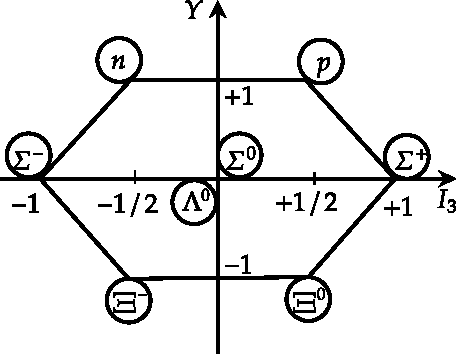
\includegraphics[height=4.7cm,width=6cm]{NP-14}
\end{figure}
The figure below shows the 8 member super multiplets of spin 0 mesons.
\begin{figure}[H]
	\centering
	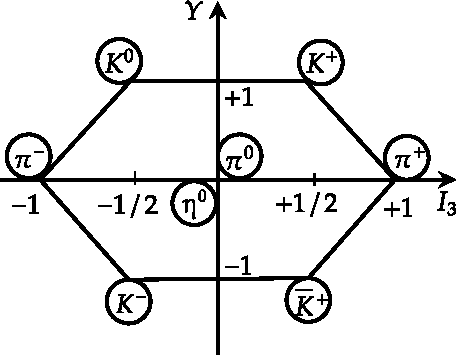
\includegraphics[height=4.7cm,width=6cm]{NP-15}
\end{figure}
The figure below shows the 10 member super multiplet of spin $\frac{3}{2}$ Baryon.
\begin{figure}[H]
	\centering
	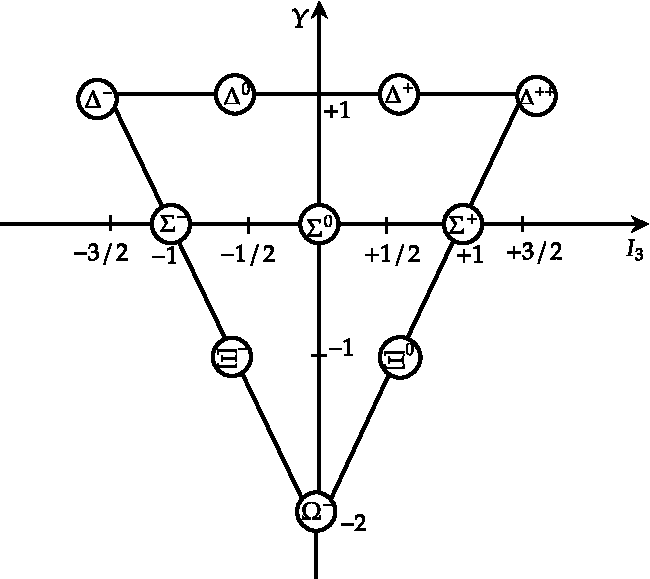
\includegraphics[height=7.2cm,width=8cm]{NP-16}
	\caption{}
	\label{}
\end{figure}
\subsubsection{Gellmann-Nishijima Relation}
$q=I_3+\frac{1}{2}(B+S)$
\section{Quark Model of Hadrons (Baryons and Mesons)}
Murray Gell-Man and G.Zweig proposed the quark model in 1964. The theory is based on the idea that the hadrons are built up from a limited number of "fundamental" units, which have acquired the name quarks. The original three quarks were labeled $u$ (for "up"), $d$ (for "down") and $s$ (for "strange").\\\\
\renewcommand*{\arraystretch}{1.5}
\begin{tabular}{|c|c|c|c|c|c|c|c|}
	\hline Quark & Charge & Spin & B & S & I & $\mathbf{I}_3$ & $\mathbf{Y}$ \\
	\hline$u$-quark & $+2 / 3 e$ & $1 / 2$ & $1 / 3$ & 0 & $1 / 2$ & $1 / 2$ & $1 / 3$ \\
	\hline$d$-quark & $-1 / 3 e$ & $1 / 2$ & $1 / 3$ & 0 & $1 / 2$ & $-1 / 2$ & $1 / 3$ \\
	\hline s-quark & $-1 / 3 e$ & $1 / 2$ & $1 / 3$ & $-1$ & 0 & 0 & $-2 / 3$ \\
	\hline
\end{tabular}\\\\
Each quark has a baryon number of $B=1 / 3$. Also each quark has an anti-quark associated with it $(\bar{u}, \bar{d} \& \bar{s})$. The magnitudes of each of the quantum number for the anti-quarks has the same magnitude as those for the quarks, but the sign is changed and Baryon is reversed.
\subsubsection{Anti-Quark Quantum Number:}
\vspace{0.3cm}
\renewcommand*{\arraystretch}{1.5}
\begin{tabular}{|c|c|c|c|c|c|c|c|}
	\hline Quark & Charge & Spin & B & S & I & $\mathbf{I}_3$ & $\mathbf{Y}$ \\
	\hline $\bar{u}$ & $-2 / 3 e$ & $1 / 2$ & $-1 / 3$ & 0 & $1 / 2$ & $-1 / 2$ & $-1 / 3$ \\
	\hline $\bar{d}$ & $+1 / 3 e$ & $1 / 2$ & $-1 / 3$ & 0 & $1 / 2$ & $+1 / 2$ & $-1 / 3$ \\
	\hline $\bar{s}$ & $+1 / 3 e$ & $1 / 2$ & $-1 / 3$ & $+1$ & 0 & 0 & $+2 / 3$ \\
	\hline
\end{tabular}\\
\subsubsection{Composition of Baryons According to Quark Model}
A baryon is made up of 3 quarks.\\
e.g. The proton is made up of two $u$-quarks and a $d$-quark (uud). Hence,\\ Electric charge of proton $=+2 / 3+2 / 3-1 / 3=+1$\\
Baryon number of proton $=+1 / 3+1 / 3+1 / 3=+1$\\
Strangeness number of proton $=0+0+0=0$\\
All are in agreement with the quantum numbers for proton.
\subsubsection{Quantum Number and Quark Contents}
\subsubsection{Baryon: 1/2 spin}
\renewcommand*{\arraystretch}{1.5}
\begin{tabular}{|c|c|c|c|c|c|c|}
	\hline Particle & Quark Content & I & I $_{\mathbf{3}}$ & Y & B & S \\
	\hline $\mathrm{p}$ & uud & $1 / 2$ & $1 / 2$ & 1 & 1 & 0 \\
	\hline $\mathrm{n}$ & udd & $1 / 2$ & $-1 / 2$ & 1 & 1 & 0 \\
	\hline $\sum^{+}$ & uus & 1 & 1 & 0 & 1 & $-1$\\
	\hline $\Sigma^0$ & $\frac{s u d+s d u}{\sqrt{2}}$ & 1 & 0 & 0 & 1 & $-1$ \\
	\hline $\sum^{-}$ & dds & 1 & $-1$ & 0 & 1 & $-1$ \\
	\hline $\Xi^0$ & uss & $1 / 2$ & $1 / 2$ & $-1$ & 1 & $-2$ \\
	\hline $\Xi^{-}$ & $\mathrm{dss}$ & $1 / 2$ & $-1 / 2$ & $-1$ & 1 & $-2$ \\
	\hline $\Lambda^{\circ}$ & $\frac{s d u-s u d}{\sqrt{2}}$ & 0 & 0 & 0 & 1 & $-1$ \\
	\hline
\end{tabular}
\subsubsection{(ii) Baryon: 3 / 2 spin}
\begin{tabular}{|c|c|c|c|c|c|c|}
	\hline Particle & Quark Content & $\mathbf{I}$ & $\mathbf{I}_{\mathbf{3}}$ & $\mathbf{Y}$ & $\mathbf{B}$ & $\mathbf{S}$ \\
	\hline$\Delta^{-}$ & $d d d$ & $3 / 2$ & $-3 / 2$ & 1 & 1 & 0 \\
	\hline$\Delta^0$ & $d d u$ & $3 / 2$ & $-1 / 2$ & 1 & 1 & 0 \\
	\hline$\Delta^{+}$ & $d u u$ & $3 / 2$ & $+1 / 2$ & 1 & 1 & 0 \\
	\hline$\Delta^{++}$ & $u u u$ & $3 / 2$ & $+3 / 2$ & 1 & 1 & 0 \\
	\hline$\Omega^{-}$ & $s s s$ & 0 & 0 & $-2$ & 1 & $-3$ \\
	\hline
\end{tabular}\\\\
Mesons are made up of one quark and one anti-quark.\\
A $\pi^{+}$meson is a combination of a u-quark and a d-anti-quark $(u \bar{d})$.\\
Electric charge of $\pi^{+}=+2 / 3+1 / 3=+1$\\
Baryon number of $\pi^{+}=+1 / 3-1 / 3=0$\\
Strangeness number of $\pi^{+}=0+0=0$\\
All these are in agreement with the quantum numbers for the $\pi^{+}$meson.\\
\renewcommand*{\arraystretch}{1.5}
\begin{tabular}{|c|c|c|c|c|c|c|}
	\hline Particle & Quark Content & $\mathbf{I}$ & $\mathbf{I}_3$ & $\mathbf{Y}$ & $\mathbf{B}$ & $\mathbf{S}$ \\
	\hline$\pi^{+}$ & $\bar{d} u$ & 1 & 1 & 0 & 0 & 0 \\
	\hline$\pi^0$ & $\frac{(u \bar{u}-d \bar{d})}{\sqrt{2}}$ & 1 & 0 & 0 & 0 & 0 \\
		\hline$\pi^{-}$ & $\bar{u} d$ & 1 & $-1$ & 0 & 0 & 0 \\
		\hline $\mathrm{K}^{+}$ & $\bar{s} u$ & $1 / 2$ & $1 / 2$ & 1 & 0 & 1 \\
		\hline $\mathrm{K}^0$ & $\bar{s} d$ & $1 / 2$ & $-1 / 2$ & 1 & 0 & 1 \\
		\hline $\mathrm{K}^{-}$ & $s \bar{u}$ & $1 / 2$ & $-1 / 2$ & $-1$ & 0 & $-1$ \\
		\hline$\overline{\mathrm{K}}^0$ & $s \bar{d}$ & $1 / 2$ & $1 / 2$ & $-1$ & 0 & $-1$ \\\hline
\end{tabular}
\subsubsection{Charm, Bottom and Top}
In 1970, the existence of a fourth quark, called "c" or charmed quark was proposed. The charmed quark was suggested to explain the suppression of certain decay process that is not observed. The charm quark has a charge of $+\frac{2}{3} e$, strangeness 0 and a charm quantum number of $+1$. Other quarks have 0 charm.\\\\
Later on two more quarks were proposed named ' $t$ ' or top quark and 'b' or bottom quark. ' $t$ ' quark has electric charge $+\frac{2}{3} e$ and 'b' quark has electric charge $-\frac{1}{3} e$.
\subsubsection{Three generation of quarks and leptons:}
Both leptons and quarks appear to come in three generations of doublets with all particles having spin $1 / 2$. The table below shows the properties of the three generations of quarks and leptons. The first generation contains two leptons, the electron and the electron-neutrino, and two quarks up and down. All properties of ordinary matter can be understood on the basis of these particles. The second generation includes the muon and muon-neutrino and the charm and strange quarks. These particles are responsible for most of the unstable particles and resonances created in high energy collisions. The third generation includes the tau and tau-neutrino and the top and bottom quarks.\\
\renewcommand*{\arraystretch}{1.5}
\begin{tabular}{|c|c|c|c|c|c|c|}
	\hline
	\multirow{7}{*}{Quark}&Generation&Quark&Symbol&Charge&Strangeness&Charm\\\hline
	&\multirow{2}{*}{1}&Up&u&$+\frac{2}{3} e$&0&0\\\cline{3-7}
	&&Down&d&$-\frac{1}{3} e$&0&0\\\cline{2-7}
	&\multirow{2}{*}{2}&Charm&c&$+\frac{2}{3} e$&0&+1\\\cline{3-7}
	&&Strange&s&$-\frac{1}{3} e$&-1&0\\\cline{2-7}
	&\multirow{2}{*}{3}&Top&t&$+\frac{2}{3} e$&0&0\\\cline{3-7}
	&&Bottom&b&$-\frac{1}{3} e$&0&0\\\cline{1-7}
\end{tabular}

\begin{tabular}{|c|c|c|c|c|}
	\multirow{6}{*}{Lepton}&Generation&Lepton&Symbol&Charge\\\cline{2-5}
	&\multirow{2}{*}{1}&Electron&$e^-$&-1\\\cline{3-5}
	&&e-neutrino&$v_e$&0\\\cline{2-5}
	&\multirow{2}{*}{2}&Meson&$\mu^-$&-1\\\cline{3-5}
	&&$\mu$-neutrino&$v_\mu$&0\\\cline{2-5}
	&3&Tau&$\tau^-$&-1\\\hline
\end{tabular}
\newpage
\begin{abox}
Practice Set-1
\end{abox}
\begin{enumerate}
	\item  Consider the decay $A \rightarrow B+C$ of a relativistic spin $-\frac{1}{2}$ particle $A$. Which of the following statements is true in the rest frame of the particle $A$ ?
{\exyear{ NET/JRF (JUNE-2019)}}	
	 \begin{tasks}(1)
		\task[\textbf{a.}]The spin of both $B$ and $C$ may be $\frac{1}{2}$
		\task[\textbf{b.}]The sum of the masses of $B$ and $C$ is greater than the mass of $A$
		\task[\textbf{c.}]The energy of $B$ is uniquely determined by the masses of the particles
		\task[\textbf{d.}]  The spin of both $B$ and $C$ may be integral
	\end{tasks}
	\item  The charm quark $S$ assigned a charm quantum number $C=1$. How should the Gellmann-Nishijima formula for electric charge be modified for four flavors of quarks?
	{\exyear{ NET/JRF (JUNE-2015)}}
	 \begin{tasks}(2)
		\task[\textbf{a.}]$I_3+\frac{1}{2}(B-S-C)$
		\task[\textbf{b.}]$I_3+\frac{1}{2}(B-S+C)$
		\task[\textbf{c.}] $I_3+\frac{1}{2}(B+S-C)$
		\task[\textbf{d.}]$I_3+\frac{1}{2}(B+S+C)$ 
	\end{tasks}
	\item  A spin-1/2 particle $A$ undergoes the delay $A \rightarrow B+C+D$, where it is known that $B$ and $C$ are also spin-1/2 particles. The complete set of allowed values of the spin of the particle $D$ is
	{\exyear{ NET/JRF (JUNE-2013)}}
	 \begin{tasks}(2)
		\task[\textbf{a.}]$\frac{1}{2}, 1, \frac{3}{2}, 2, \frac{5}{2}, 3, \ldots$
		\task[\textbf{b.}]0,1
		\task[\textbf{c.}]$\frac{1}{2}$ only
		\task[\textbf{d.}]$\frac{1}{2}, \frac{3}{2}, \frac{5}{2}, \frac{7}{2}, \ldots$ 
	\end{tasks}
	\item  A baryon $X$ decays by strong interaction as $X \rightarrow \Sigma^{+}+\pi^{-}+\pi^0$, where $\Sigma^{+}$is a member of the isotriplet $\left(\Sigma^{+}, \Sigma^0, \Sigma^{-}\right)$. The third component $I_3$ of the isospin of $X$ is
	{\exyear{ NET/JRF (JUNE-2017)}}
	 \begin{tasks}(4)
		\task[\textbf{a.}]0
		\task[\textbf{b.}] $1 / 2$
		\task[\textbf{c.}]1
		\task[\textbf{d.}] $3 / 2$
	\end{tasks}
	\item  The reaction ${ }_1^2 D+{ }_1^2 D \rightarrow{ }_2^4 \mathrm{He}+\pi^0$ cannot proceed via strong interactions because it violates the conservation of
	{\exyear{ NET/JRF (JUNE-2015)}}
	 \begin{tasks}(2)
		\task[\textbf{a.}]Angular momentum
		\task[\textbf{b.}]Electric charge
		\task[\textbf{c.}]Baryon number
		\task[\textbf{d.}] Isospin 
	\end{tasks}

	\item  A beam of pions $\left(\pi^{+}\right)$is incident on a proton target, giving rise to the process
	$$
	\pi^{+}+p \rightarrow n+\pi^{+}+\pi^{+}
	$$
	Assuming that the decay proceeds through strong interactions, the total isospin $I$ and its third component $I_3$ for the decay products, are
	{\exyear{ NET/JRF (JUNE-2011)}}
	 \begin{tasks}(2)
		\task[\textbf{a.}] $I=\frac{3}{2}, I_3=\frac{3}{2}$
		\task[\textbf{b.}]$I=\frac{5}{2}, I_3=\frac{5}{2}$
		\task[\textbf{c.}]$I=\frac{5}{2}, I_3=\frac{3}{2}$
		\task[\textbf{d.}] $I=\frac{1}{2}, I_3=-\frac{1}{2}$
	\end{tasks}
	\item  A beam of pions $\left(\pi^{+}\right)$is incident on a proton target, giving rise to the process
	$$
	\pi^{+}+p \rightarrow n+\pi^{+}+\pi^{+}
	$$
	Using isospin symmetry, the cross-section for the above process can be related to that of the process
	 \begin{tasks}(2)
		\task[\textbf{a.}]$\pi^{-} n \rightarrow p \pi^{-} \pi^{-}$
		\task[\textbf{b.}]$\pi^{-} \bar{p} \rightarrow \bar{n} \pi^{-} \pi^{-}$
		\task[\textbf{c.}]$\pi^{+} n \rightarrow p \pi^{+} \pi^{-}$
		\task[\textbf{d.}]  $\pi^{+} \bar{p} \rightarrow n \pi^{+} \pi^{-}$
	\end{tasks}

	\item  The dominant interactions underlying the following processes
	A. $K^{-}+p \rightarrow \sum^{-}+\pi^{+}$, B. $\mu^{-}+\mu^{+} \rightarrow K^{-}+K^{+}$, C. $\Sigma^{+} \rightarrow p+\pi^0$ are
	{\exyear{ NET/JRF (JUNE-2012)}}
	 \begin{tasks}(1)
		\task[\textbf{a.}]A: strong, B: electromagnetic and; C: weak
		\task[\textbf{b.}]A: strong, B: weak and; C: weak
		\task[\textbf{c.}]A: weak, B: electromagnetic and; C: strong
		\task[\textbf{d.}]  A: weak, B: electromagnetic and; C: weak
	\end{tasks}
	
	\item  Consider the four processes\\
	(i) $p^{+} \rightarrow n+e^{+}+v_e$\\
	(ii) $\Lambda^0 \rightarrow p^{+}+e^{+}+v_e$\\
	(iii) $\pi^{+} \rightarrow e^{+}+v_e$\\
	(iv) $\pi^0 \rightarrow \gamma+\gamma$\\
	which of the above is/are forbidden for free particles?
	{\exyear{NET/JRF (DEC-2014)}}
	 \begin{tasks}(2)
		\task[\textbf{a.}]Only (ii)
		\task[\textbf{b.}](ii) and (iv)
		\task[\textbf{c.}](i) and (iv)
		\task[\textbf{d.}]  (i) and (ii)
	\end{tasks}

	\item  Consider the following processes involving free particles\\
	(i) $\bar{n} \rightarrow \bar{p}+e^{+}+\bar{v}_e$\\
	(ii) $\bar{p}+n \rightarrow \pi^{-}$\\
	(iii) $p+n \rightarrow \pi^{+}+\pi^0+\pi^0$\\
	(iv) $p+\bar{v}_e \rightarrow n+e^{+}$\\
	Which of the following statements is true?
	{\exyear{ NET/JRF (DEC-2015)}}
	 \begin{tasks}(1)
		\task[\textbf{a.}] Process (i) obeys all conservation laws
		\task[\textbf{b.}]Process (ii) conserves baryon number, but violates energy-momentum conservation
		\task[\textbf{c.}] process (iii) is not allowed by strong interaction but is allowed by weak interactions
		\task[\textbf{d.}] Process (iv) conserves baryon number, but violates lepton number conservation
	\end{tasks}
	
	\item Which of the following reaction(s) is/are allowed by the conservation laws?
	(i) $\pi^{+}+n \rightarrow \Lambda^0+K^{+}$
	(ii) $\pi^{-}+p \rightarrow \Lambda^0+K^0$
	{\exyear{ NET/JRF (DEC-2016)}}
	 \begin{tasks}(2)
		\task[\textbf{a.}]Both (i) and (ii)
		\task[\textbf{b.}] Only (i)
		\task[\textbf{c.}] Only (ii)
		\task[\textbf{d.}]  Neither (i) nor (ii)
	\end{tasks}

	\item  Which of the following process is not allowed by the strong interaction but is allowed by the weak interaction?
	{\exyear{ NET/JRF (DEC-2017)}}
	 \begin{tasks}(2)
		\task[\textbf{a.}]$K^0+\pi^0 \rightarrow \bar{K}^0+\pi^{+}+\pi^{-}$
		\task[\textbf{b.}]$p+n \rightarrow d+p+\bar{p}$
		\task[\textbf{c.}]$\Delta^{+}+K^0 \rightarrow p+n$
		\task[\textbf{d.}] $p+\Delta^{+} \rightarrow \bar{n}+\Delta^{++}$
	\end{tasks}

	\item  Which of the following elementary particle processes does not conserve strangeness?
	{\exyear{ NET/JRF (JUNE-2018)}}
	 \begin{tasks}(2)
		\task[\textbf{a.}]$\pi^0+p \rightarrow k^{+}+\wedge^0$
		\task[\textbf{b.}]$\pi^{-}+p \rightarrow k^0+\wedge^0$
		\task[\textbf{c.}]$\Delta^0 \rightarrow \pi^0+n$
		\task[\textbf{d.}] $K^0 \rightarrow \pi^{+}+\pi^{-}$
	\end{tasks}

	\item  Which of the following decay processes is allowed?
	 \begin{tasks}(2)
		\task[\textbf{a.}]$K^0 \rightarrow \mu^{+}+\mu^{-}$
		\task[\textbf{b.}] $\mu^{-} \rightarrow e^{-}+\gamma$
		\task[\textbf{c.}]$n \rightarrow p+\pi^{-}$
		\task[\textbf{d.}] $n \rightarrow \pi^{+}+\pi^{-}$
	\end{tasks}

	\item  The recently-discovered Higgs boson at the LHC experiment has a decay mode into a photon and a $Z$ boson. If the rest masses of the Higgs and $Z$ boson are $125 \mathrm{GeV} / \mathrm{c}^2$ and $90 \mathrm{GeV} / \mathrm{c}^2$ respectively, and the decaying Higgs particle is at rest, the energy of the photon will approximately be
	{\exyear{ NET/JRF (JUNE-2014)}}
	 \begin{tasks}(2)
		\task[\textbf{a.}] $35 \sqrt{3} \mathrm{GeV}$
		\task[\textbf{b.}]$35 \mathrm{GeV}$
		\task[\textbf{c.}] $30 \mathrm{GeV}$
		\task[\textbf{d.}] $15 \mathrm{GeV}$
	\end{tasks}

	\item  In the large hadron collider $(L H C)$, two equal energy proton beams traverse in opposite directions along a circular path of length $27 \mathrm{~km}$. If the total centre of mass energy of a proton-proton pair is $14 \mathrm{TeV}$, which of the following is the best approximation for the proper time taken by a proton to traverse the entire path?
	{\exyear{ NET/JRF (JUNE-2016)}}
	 \begin{tasks}(4)
		\task[\textbf{a.}]$12 n s$
		\task[\textbf{b.}]$1.2 \mu \mathrm{s}$
		\task[\textbf{c.}]$1.2 \mathrm{~ns}$
		\task[\textbf{d.}] $0.12 \mu \mathrm{s}$ 
	\end{tasks}

	\item  Muons are produced through the annihilation of particle $a$ and its anti-particle, namely the process $a+\bar{a} \rightarrow \mu^{+}+\mu^{-}$. A muon has a rest mass of $105 \mathrm{MeV} / \mathrm{c}^2$ and its proper life time is $2 \mu \mathrm{s}$. If the center of mass energy of the collision is $2.1 \mathrm{GeV}$ in the laboratory frame that coincides with the center-of-mass frame, then the fraction of muons that will decay before they reach a detector placed $6 \mathrm{~km}$ away from the interaction point is
	{\exyear{ NET/JRF (JUNE-2013)}}
	 \begin{tasks}(4)
		\task[\textbf{a.}]$e^{-1}$
		\task[\textbf{b.}]$1-e^{-1}$
		\task[\textbf{c.}] $1-e^{-2}$
		\task[\textbf{d.}]  $e^{-10}$
	\end{tasks}

	\item  In a classical model, a scalar (spin-0) meson consists of a quark and an antiquark bound by a potential $V(r)=a r+\frac{b}{r}$, where $a=200 \mathrm{MeV} \mathrm{fm}^{-1}$ and $b=100 \mathrm{MeV} \mathrm{fm}$. If the masses of the quark and antiquark are negligible, the mass of the meson can be estimated as approximately
	{\exyear{ NET/JRF (JUNE-2014)}}
	 \begin{tasks}(4)
		\task[\textbf{a.}]$141 \mathrm{MeV} / \mathrm{c}^2$
		\task[\textbf{b.}] $283 \mathrm{MeV} / \mathrm{c}^2$
		\task[\textbf{c.}]$353 \mathrm{MeV} / \mathrm{c}^2$
		\task[\textbf{d.}] $425 \mathrm{MeV} / \mathrm{c}^2$
	\end{tasks}

	\item  The range of the nuclear force between two nucleons due to the exchange of pions is $1.40 \mathrm{fm}$. If the mass of pion is $140 \mathrm{MeV} / \mathrm{c}^2$ and the mass of the rho-meson is $770 \mathrm{MeV} / \mathrm{c}^2$, then the range of the force due to exchange of rho-mesons is
	{\exyear{ NET/JRF (JUNE-2017)}}
	 \begin{tasks}(4)
		\task[\textbf{a.}]$1.40 \mathrm{fm}$
		\task[\textbf{b.}]$7.70 \mathrm{fm}$
		\task[\textbf{c.}]$0.25 \mathrm{fm}$
		\task[\textbf{d.}]$0.18 \mathrm{fm}$ 
	\end{tasks}

	\item  The mean life-time of the following decays: $\rho_0 \rightarrow \pi^{+}+\pi^{-}, \pi^0 \rightarrow \gamma+\gamma, \mu^{-} \rightarrow e^{-}+\bar{v}_e+v_\mu$, are $\tau_\rho, \tau_\pi$ and $\tau_\mu$ respectively.
	They satisfy
	{\exyear{ NET/JRF (JUNE-2019)}}
	 \begin{tasks}(2)
		\task[\textbf{a.}]$\tau_\pi<\tau_\rho<\tau_\mu$
		\task[\textbf{b.}]$\tau_\mu<\tau_\rho<\tau_\pi$
		\task[\textbf{c.}]$\tau_\rho<\tau_\pi<\tau_\mu$
		\task[\textbf{d.}] $\tau_\rho<\tau_\mu<\tau_\pi$
	\end{tasks}

	\item  A particle, which is a composite state of three quarks $u, d$ and $s$, has electric charge, spin and strangeness respectively, equal to
	{\exyear{ NET/JRF (DEC-2016)}}
	 \begin{tasks}(2)
		\task[\textbf{a.}]$1, \frac{1}{2},-1$
		\task[\textbf{b.}]$0,0,-1$
		\task[\textbf{c.}]$0, \frac{1}{2},-1$
		\task[\textbf{d.}] $-1,-\frac{1}{2}+1$
	\end{tasks}

	\item  The elastic scattering of a neutrino $v_e$ by an electron $e^{-}$, i.e. the reaction $v_e+e^{-} \rightarrow v_e+e^{-}$can be described by the interaction Hamiltonian
	$$
	H_{\mathrm{int}}=\frac{1}{\sqrt{2}} G_F \int d^3 x\left(\bar{\psi}_e(x) \gamma^\mu \psi_{v e}(x)\right)\left(\bar{\psi}_{v e}(x) \gamma_\mu \psi_e(x)\right)
	$$
	The cross-section of the above process depends on the centre of mass energy $E$, as
	{\exyear{ NET/JRF (JUNE-2019)}}
	 \begin{tasks}(4)
		\task[\textbf{a.}]$\frac{1}{E^2}$
		\task[\textbf{b.}]$E^2$
		\task[\textbf{c.}]$E$
		\task[\textbf{d.}] $\sqrt{E}$
	\end{tasks}

	\item  A deuteron $d$ captures a charged pion $\pi^{-}$in the $l=1$ state, and subsequently decays into a pair of neutrons $(n)$ via strong interaction. Given that the intrinsic parities of $\pi^{-}, d$ and $n$ are $-1,+1$ and $+1$ respectively, the spin wavefunction of the final state neutrons is
	{\exyear{ NET/JRF (JUNE-2018)}}
	 \begin{tasks}(2)
		\task[\textbf{a.}]Linear combination of a singlet and a triplet
		\task[\textbf{b.}]Singlet
		\task[\textbf{c.}]Triplet
		\task[\textbf{d.}] Doublet
	\end{tasks}

	\item  Charged pions $\pi^{-}$decay to muons $\mu^{-}$and anti-muon neutrinos $\vec{v}_\mu ; \pi^{-} \rightarrow \mu^{-}+\vec{v}_\mu$. Take the rest masses of a muon and a pion to be $105 \mathrm{MeV}$ and $140 \mathrm{MeV}$, respectively. The probability that the measurement of the muon spin along the direction of its momentum is positive, is closest to
	NET/JRF (JUNE-2020)
	 \begin{tasks}(4)
		\task[\textbf{a.}]$0.5$
		\task[\textbf{b.}]$0.75$
		\task[\textbf{c.}]1
		\task[\textbf{d.}] 0
	\end{tasks}
	
	 \colorlet{ocre1}{ocre!70!}
	\colorlet{ocrel}{ocre!30!}
	\setlength\arrayrulewidth{1pt}
	\begin{table}[H]
		\centering
		\arrayrulecolor{ocre}
		\begin{tabular}{|p{1.5cm}|p{1.5cm}||p{1.5cm}|p{1.5cm}|}
			\hline
			\multicolumn{4}{|c|}{\textbf{Answer key}}\\\hline\hline
			\rowcolor{ocrel}Q.No.&Answer&Q.No.&Answer\\\hline
			1&\textbf{c} &2&\textbf{d}\\\hline 
			3&\textbf{c} &4&\textbf{a} \\\hline
			5&\textbf{d} &6&\textbf{c} \\\hline
			7&\textbf{c}&8&\textbf{a}\\\hline
			9&\textbf{d}&10&\textbf{b}\\\hline
			11&\textbf{a} &12&\textbf{a}\\\hline
			13&\textbf{d}&14&\textbf{a}\\\hline
			15&\textbf{c}&16&\textbf{a}\\\hline
			17&\textbf{b}&18&\textbf{b}\\\hline
			19&\textbf{c}&20&\textbf{c}\\\hline
			21&\textbf{c} &22&\textbf{c}\\\hline
			23&\textbf{b}&24&\textbf{c}\\\hline
		\end{tabular}
	\end{table}
	
	
	
	
	
	
	
	
	
	
	
	
	
	
	
	
	
\end{enumerate}












































































\begin{abox}
Practice Set-2
\end{abox}
\begin{enumerate}
	\item  Which one of the following sets corresponds to fundamental particles?
	 {\exyear{ 	GATE-2012}}
	 \begin{tasks}(2)
		\task[\textbf{a.}]Proton, electron and neutron
		\task[\textbf{b.}]Proton, electron and photon
		\task[\textbf{c.}]Electron, photon and neutrino
		\task[\textbf{d.}]Quark, electron and meson 
	\end{tasks}

	\item  Choose the CORRECT statement from the following
	 \begin{tasks}(1)
		\task[\textbf{a.}]Neutron interacts through electromagnetic interaction
		\task[\textbf{b.}]Electron does not interact through weak interaction
		\task[\textbf{c.}]Neutrino interacts through weak and electromagnetic interaction
		\task[\textbf{d.}] Quark interacts through strong interaction but not through weak interaction
	\end{tasks}

	\item  The isospin and the strangeness of $\Omega^{-}$baryon are
	{\exyear{ GATE-2011}}
	 \begin{tasks}(4)
		\task[\textbf{a.}]$1,-3$
		\task[\textbf{b.}]$0,-3$
		\task[\textbf{c.}]1,3
		\task[\textbf{d.}]0,3 
	\end{tasks}

	\item The isospin $(I)$ and baryon number $(B)$ of the up quark is
	{\exyear{ 	GATE-2013}}
	 \begin{tasks}(2)
		\task[\textbf{a.}]$I=1, B=1$
		\task[\textbf{b.}]$I=1, B=1 / 3$
		\task[\textbf{c.}]$I=1 / 2, B=1$
		\task[\textbf{d.}]$I=1 / 2, B=1 / 3$ 
	\end{tasks}

	\item  Which one of the following is a fermions'?
	{\exyear{ 	GATE-2014}}
	 \begin{tasks}(2)
		\task[\textbf{a.}]$\alpha$-particle
		\task[\textbf{b.}]${ }_4 B e^7$ nucleus
		\task[\textbf{c.}]Hydrogen atom
		\task[\textbf{d.}]Deuteron 
	\end{tasks}

	\item  In the decay, $\mu^{+} \rightarrow e^{+}+v_e+X$, what is $X$ ?
	{\exyear{ GATE-2018}}
	 \begin{tasks}(4)
		\task[\textbf{a.}]$\gamma$
		\task[\textbf{b.}]$\bar{v}_e$
		\task[\textbf{c.}]$v_\mu$
		\task[\textbf{d.}]$\bar{v}_\mu$ 
	\end{tasks}

	\item  The basic process underlying the neutron $\beta$-decay is
	{\exyear{ GATE-2010}}
	 \begin{tasks}(2)
		\task[\textbf{a.}]$d \rightarrow u+e^{-}+\bar{v}_e$
		\task[\textbf{b.}]$d \rightarrow u+e^{-}$
		\task[\textbf{c.}]$s \rightarrow u+e^{-}+\bar{v}_e$
		\task[\textbf{d.}]$u \rightarrow d+e^{-}+\bar{v}_e$ 
	\end{tasks}

	\item  Match the reactions on the left with the associated interactions on the right.\\
	(1) $\pi^{+} \rightarrow \mu^{+}+v_\mu$\hspace{3cm}
	(i) Strong\\
	(2) $\pi^0 \rightarrow \gamma+\gamma$\hspace{3.5cm}
	(ii) Electromagnetic\\
	(3) $\pi^0+\mathrm{n} \rightarrow \pi^{-}+\mathrm{p}$\hspace{2.6cm}
	(iii) Weak
	{\exyear{ GATE-2010}}
	 \begin{tasks}(2)
		\task[\textbf{a.}]$(1$, iii), (2, ii), (3, i)
		\task[\textbf{b.}]$(1$, i), (2, ii), (3, iii)
		\task[\textbf{c.}](1, ii), (2, i), (3, iii)
		\task[\textbf{d.}](1, iii), (2, i), (3, ii) 
	\end{tasks}

	\item  The quark content of $\Sigma^{+}, K^{-}, \pi^{-}$and $p$ is indicated:
	$$
	\left|\Sigma^{+}\right\rangle=|u u s\rangle ;\left|K^{-}\right\rangle=|s \bar{u}\rangle ;\left|\pi^{-}\right\rangle=|\bar{u} d\rangle ;|p\rangle=|u u d\rangle .
	$$
	In the process, $\pi^{-}+p \rightarrow K^{-}+\Sigma^{+}$, considering strong interactions only, which of the following statements is true?
	{\exyear{ GATE-2012}}
	 \begin{tasks}(1)
		\task[\textbf{a.}]The process, is allowed because $\Delta \mathrm{S}=0$
		\task[\textbf{b.}] The process is allowed because $\Delta \mathrm{I}_3=0$
		\task[\textbf{c.}] The process is not allowed because $\Delta \mathrm{S} \neq 0$ and $\Delta \mathrm{I}_3 \neq 0$
		\task[\textbf{d.}]The process is not allowed because the baryon number is violated 
	\end{tasks}

	\item  The decay process $n \rightarrow p^{+}+e^{-}+\bar{v}_e$ violates
	{\exyear{ 	GATE-2013}}
	 \begin{tasks}(2)
		\task[\textbf{a.}]Baryon number
		\task[\textbf{b.}] lepton number
		\task[\textbf{c.}] Isospin
		\task[\textbf{d.}] Strangeness
	\end{tasks}

	\item  Which one of the following three-quark states $(q q q)$ denoted by $X$ CANNOT be a possible baryon? The corresponding electric charge is indicated in the superscript.
	{\exyear{ 	GATE-2014}}
	 \begin{tasks}(4)
		\task[\textbf{a.}]$X^{++}$
		\task[\textbf{b.}]$\mathrm{X}^{+}$
		\task[\textbf{c.}]$X^{-}$
		\task[\textbf{d.}] $\mathrm{X}^{--}$ 
	\end{tasks}

	\item  The decay $\mu^{+} \rightarrow e^{+}+\gamma$ is forbidden, because it violates
	{\exyear{ 	GATE-2015}}
	 \begin{tasks}(1)
		\task[\textbf{a.}] Momentum and lepton number conservations
		\task[\textbf{b.}]Baryon and lepton number conservations
		\task[\textbf{c.}]Angular momentum conservation
		\task[\textbf{d.}]  Lepton number conservation
	\end{tasks}

	\item  In the $S U(3)$ quark model, the triplet of mesons $\left(\pi^{+}, \pi^0, \pi^{-}\right)$has
	{\exyear{ GATE-2016}}
	 \begin{tasks}(2)
		\task[\textbf{a.}]Isospin $=0$, Strangeness $=0$
		\task[\textbf{b.}] Isospin $=1$, Strangeness $=0$
		\task[\textbf{c.}]Isospin $=\frac{1}{2}$, Strangeness $=+1$
		\task[\textbf{d.}]  Isospin $=\frac{1}{2}$, Strangeness $=-1$
	\end{tasks}

	\item  Which one of the following conservation laws is violated in the decay $\tau^{+} \rightarrow \mu^{+} \mu^{+} \mu^{-}$
	{\exyear{ GATE-2017}}
	 \begin{tasks}(2)
		\task[\textbf{a.}]Angular momentum
		\task[\textbf{b.}]Total Lepton number
		\task[\textbf{c.}]Electric charge
		\task[\textbf{d.}]Tau number 
	\end{tasks}

	\item  The elementary particle $\Xi^0$ is placed in the baryon decuplet, shown below, at
		{\exyear{GATE-2018}}
	\begin{figure}[H]
		\centering
		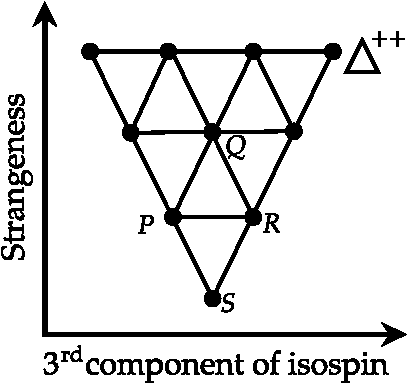
\includegraphics[height=4cm,width=4.5cm]{NP-13}
	\end{figure}
	 \begin{tasks}(4)
		\task[\textbf{a.}]$P$
		\task[\textbf{b.}]$Q$
		\task[\textbf{c.}]$R$
		\task[\textbf{d.}] $S$ 
	\end{tasks}

	\item  Considering baryon number and lepton number conservation laws, which of the following process is/are allowed?
	(i) $p \rightarrow \pi^0+e^{+}+v_e$\hspace{2cm}
	(ii) $e^{+}+v_e \rightarrow \mu^{+}+v_\mu$
	{\exyear{ 	GATE-2019}}
	 \begin{tasks}(2)
		\task[\textbf{a.}]Both (i) and (ii)
		\task[\textbf{b.}]Only (i)
		\task[\textbf{c.}]Only (ii)
		\task[\textbf{d.}]Neither (i) nor (ii)
	\end{tasks}
\begin{answer}
	\begin{align*}
	 &\text{(i) }\quad p \rightarrow \pi^0+e^{+}+v_e\\
	&B: \quad+1 \quad 0 \quad 0 \quad 0:\text{ Not conserved}\\ 
	&\text{Therefore, this is not an allowed process}\\
	&\text{(II)}\quad e^{+}+v_e \quad \rightarrow \quad \mu^{+}+v_\mu\\
	&\begin{array}{lclcc}
	q: & +1 & 0 & +1 & 0: \text { conserved } \\
	\text { spin: } & 1 / 2 & 1 / 2 & 1 / 2 & 1 / 2: \text { conserved } \\
	L_e: & -1 & +1 & 0 & 0: \text { conserved } \\
	L_\mu: & 0 & 0 & -1 & +1: \text { conserved }
	\end{array}\\
	&\text{Since neutrino is involved, therefore parity is violated. This is allowed through weak interaction.}
	\end{align*}
		So the correct answer is \textbf{Option (c)}
\end{answer}
	\item  A massive particle $X$ in free space decays spontaneously into two photons. Which of the following statements is true for $X$ ?
{\exyear{ 	GATE-2019}}
	 \begin{tasks}(1)
		\task[\textbf{a.}] $X$ is charged
		\task[\textbf{b.}]Spin of $X$ must be greater than or equal to 2
		\task[\textbf{c.}]$X$ is a boson
		\task[\textbf{d.}]$X$ must be a baryon 
	\end{tasks}

	\item  Low energy collision ( $s$-wave scattering) of pion $\left(\pi^{+}\right)$with deuteron $(d)$ results in the production of two proton $\left(\pi^{+}+d \rightarrow p+p\right)$. The relative orbital angular momentum (in units of $\hbar$ ) of the resulting two-proton system for this reaction is
	{\exyear{ GATE-2019}}
	 \begin{tasks}(4)
		\task[\textbf{a.}]0
		\task[\textbf{b.}]1
		\task[\textbf{c.}]2
		\task[\textbf{d.}] 3
	\end{tasks}

	\item  A particle $Y$ undergoes strong decay $Y \rightarrow \pi^{-}+\pi^{-}$. The isospin of $Y$ is---------
	{\exyear{ GATE- 2020}}

	\item  A particle $X$ is produced in the process $\pi^{+}+p \rightarrow K^{+}+X$ via the strong interaction. If the quark content of the $K^{+}$is $u \bar{s}$, the quark content of $X$ is
{\exyear{	GATE- 2020}}
	 \begin{tasks}(4)
		\task[\textbf{a.}]$c \bar{s}$
		\task[\textbf{b.}]und
		\task[\textbf{c.}]uus
		\task[\textbf{d.}]$u \bar{d}$ 
	\end{tasks}

\end{enumerate}
 \colorlet{ocre1}{ocre!70!}
\colorlet{ocrel}{ocre!30!}
\setlength\arrayrulewidth{1pt}
\begin{table}[H]
	\centering
	\arrayrulecolor{ocre}
	\begin{tabular}{|p{1.5cm}|p{1.5cm}||p{1.5cm}|p{1.5cm}|}
		\hline
		\multicolumn{4}{|c|}{\textbf{Answer key}}\\\hline\hline
		\rowcolor{ocrel}Q.No.&Answer&Q.No.&Answer\\\hline
		1&\textbf{a} &2&\textbf{d}\\\hline 
		3&\textbf{b} &4&\textbf{d} \\\hline
		5&\textbf{b} &6&\textbf{d} \\\hline
		7&\textbf{a}&8&\textbf{a}\\\hline
		9&\textbf{c}&10&\textbf{c}\\\hline
		11&\textbf{d} &12&\textbf{d}\\\hline
		13&\textbf{b}&14&\textbf{d}\\\hline
		15&\textbf{c}&16&\textbf{c} \\\hline
		17&\textbf{c}&18&\textbf{b}\\\hline
		19&\textbf{2}&20&\textbf{c}\\\hline
	\end{tabular}
\end{table}
\begin{abox}
Practice Set-3
\end{abox}
\begin{enumerate}
	\item  Particles $X$ and $Y$ can be produced by strong interaction
	$$
	\begin{aligned}
	&K^{-}+p \rightarrow K^{+}+X \\
	&K^{-}+p \rightarrow \pi^0+Y
	\end{aligned}
	$$
	identify the particles $X(1321 \mathrm{MeV})$ and $Y(1192 \mathrm{MeV})$ and deduce their quark content.
		\begin{answer}
		\begin{align*}
		&\text { (i) } K^{-}+p \rightarrow K^{+}+X\\
		&\begin{array}{lllll}
q:&-1&+1&+1&(-1)\\
\text { Spin: } &\ 0&\frac{1}{2} & 0 & \frac{1}{2}\\
B: &\ 0 &+1 & 0 &(+1)\\
S:&-1 & 0 & +1 & (-2)
		\end{array}\\
	&\text{	The particle $X$ is $X i$-hyper on $\left(\Xi^{-}\right)$. The quark content of $\Xi^{-}$is $d s s$}\\
		&\text{(ii) $\quad K^{-}+p \rightarrow \pi^0+Y$}\\
		&\begin{array}{lllll}
	q:&-1 &+1 & 0 &(0)\\
	\text{Spin: }&0 & \frac{1}{2} & 0 & \frac{1}{2}\\
	B: &0 &+1 & 0 &(+1)\\
	S: & -1 & 0 & 0 & (-1)
		\end{array}\\
		&\text { Therefore the particle } Y \text { is sigma hyperon }\left(\Sigma^0\right) \text {. The quark content of }\left(\Sigma^0\right) \text { is } u d s \text {. }
		\end{align*}
	\end{answer}
	\item  Which of the following processes are allowed in electromagnetic interaction and which one allowed in weak interaction via the exchange of a single $W^{\pm}$or $Z^0$ ?\\
	(a) $K^{+} \rightarrow \pi^0+e^{+}+v_e$\\
	(b) $\Sigma^0 \rightarrow \Lambda+v_e+\bar{v}_e$
		\begin{answer}
		\begin{align*}
		&\text { (a) } K^{+} \rightarrow \pi^0+e^{+}+v_e\\
		&\begin{array}{lllll}
		q:&+1&0&+1 & 0:\text{ Conserved}\\
		\text{Spin: }&0 & 0 & \frac{1}{2} & \frac{1}{2}: \text{ Conserved}\\
		I: & \frac{1}{2} & 1 & 0 & 0:\text{ Not Conserved}\\
		I_3: & \frac{1}{2} & 0 & 0 & 0:\text{ Not Conserved}\\
		\operatorname{Str} S:&+1 & 0 & 0 & 0: \text { Not Conserved }
		\end{array}
		\intertext{It is forbidden as electromagnetic interaction because $\Delta S \neq 0$ and also forbidden as weak interaction because there is no strangeness changing current.}
		&\text { (b) } \quad \Sigma^0 \rightarrow \Lambda+v_e+\bar{v}_e\\
		&\begin{array}{lllll}
		S:& 0 &0 & 0 & 0:\text{ Conserved}\\
		\text{Spin: }&\frac{1}{2} & \frac{1}{2} & \frac{1}{2} & \frac{1}{2}:\text{ Conserved}\\
		L_e:& 0&0&+1&-1:\text{ Conserved}\\
		B:&+1&+1& 0 &0:\text{ Conserved}\\
		I: &1 & 0 & 0 & 0:\text{ Conserved}\\
		I_3: & 1 & 0 & 0 & 0:\text{ Conserved}\\
		S:&-1 &-1 & 0 & 0:\text{ Conserved}\\
		\end{array}\\
		&\text{It is allowed as electromagnetic interaction}
		\end{align*}
	\end{answer}
	\item   A particle $X$ decays at rest weakly as follows $X \rightarrow \pi^0+\mu^{+}+v_\mu$ identify the particle $X$ and give its quark content.
			\begin{answer}
		\begin{align*}
		&X \rightarrow \pi^0+\mu^{+}+v_\mu\\
		&\begin{array}{lllll}
		q: &(+1) & 0&+1 & 0:\text{ Conserved}\\
		\text{	Spin:}& (0): & 0 & \frac{1}{2} & \frac{1}{2}:\text{ Conserved}\\
		L: &(0) &0 &-1 &+1\text{ : Conserved}\\
		B: &(0) & 0 & 0 & 0:\text{ Conserved}\\
		I: &(1 / 2) & 1 & 0 & 0\text{ : Must violate}\\
		I_3:&(\pm 1 / 2) & 0 & 0 & 0:\text{ Must violate}\\
		S: &(\pm 1) & 0 & 0 &0:\text{ Must change}\text { by } \Delta S=\pm 1
		\end{array}\\
		&\text { Therefore, the particle } X \text { is } K^{+} \text {-meson. The quark content of } K^{+} \text {- meson is } u \bar{s}
		\end{align*}
	\end{answer}
	\item (a) What are the quark constituents of the states $\Delta^{-}, \Delta^0, \Delta^{+}, \Delta^{++}$\\
	(b) Assuming the quarks are in the states of zero angular momentum, what fundamental difficulty appears to be associated with the $\Delta$ state, which has $I=3 / 2$ and how it is resolved?
		\begin{answer}
		(a) $\Delta^{-}: d d d, \Delta^0: d d u, \Delta^{+}: u u d, \Delta^{++}: u u u$\\	
	(b) The fundamental difficulty is that Pauli's principle is violated. For example consider the spin at $\Delta^{-}$. All the three $d$-quarks have to be aligned with the same $j_z=-\frac{1}{2}$. The same difficulty arises for $\Delta^{++}$. The difficulty is removed by endowing a new intrinsic quantum number (color) to the quarks. Thus, the three $d$-quarks in $\Delta^{-}$or the three $u-$ quarks in $\Delta^{++}$differ in color, Red $(R)$, Green $(\mathrm{G})$, and Blue (B).
	\end{answer}
	\item Use the quark model to determine the quark composition of\\
	(a) $\Sigma^{+}, \Sigma^{-}, n$ and $p$\\
	(b) $K^{+}, K^{-}, \pi^{+}, \pi^{-}$
	\begin{answer}
	\begin{align*}
\text{(a)} \quad \Sigma^{+}: u u s, \Sigma^{-}: d d s, n: u d d, p: u u d\\
\text{(b)} \quad  K^{+}: u \bar{s}, K^{-}: d s, \pi^{+}: u \bar{d}, \pi^{-}: \bar{u} d
	\end{align*}
\end{answer}
	\item Which of the following reaction are allowed and which forbidden as under weak interaction?
	 \begin{tasks}(2)
		\task[\textbf{a.}] $v_\mu+p \rightarrow \mu^{+}+\eta$
		\task[\textbf{b.}]$v_e+p \rightarrow e^{-}+\pi^{+}+p$
		\task[\textbf{c.}]$K^{+} \rightarrow \pi^0+\mu^{+}+v_\mu$
		\task[\textbf{d.}] $\Lambda \rightarrow \pi^{+}+e^{-}+\bar{v}_e$
	\end{tasks}
	\begin{answer}
(a) Forbidden because Lepton number is not conserved\\
	(b) Forbidden because charge is not conserved\\
	(c) Allowed\\
	(d) Allowed
\end{answer}
	\item (a) Write the Gellmann's equation for quarks. Are quarks observed as free particle?\\
	(b) Write the quark content of $D^{+}$- meson and $\pi^0$-meson.
		\begin{answer}
				(a) Gellmann's equation is generalized as
		\begin{align*}
		&\frac{Q}{e}=I_3+\frac{1}{2}\left(B+S+C+B^*+T\right)\\
	&\text{	where $B$ denotes Baryon number, $S$ the strangeness, $C$ the charm, $B^*$ the beauty of bottom }\\
	&\text{and $T$ the top.}\\
	&\text{	Quarks are not observed as free particle as they are confined in Hardons}\\
	&\text{(b)}\quad  D^{+}: c \bar{d}\\
	&\pi^0: \frac{u \bar{u}-\bar{d} \bar{d}}{\sqrt{2}}
		\end{align*}
	\end{answer}
	\item Indicate how the following quantities will transform under the $P$ (space inversion) and $T$ (time reversal) operation:
	 \begin{tasks}(2)
		\task[\textbf{a.}] Position coordinate $(\vec{r})$
		\task[\textbf{b.}] Momentum vector $(\vec{p})$
		\task[\textbf{c.}] Electric field $(\vec{E})$
		\task[\textbf{d.}] Magnetic field $(\vec{B})$
	\end{tasks}
		\begin{answer}
		\begin{align*}
		\text { (a) } p: \vec{r}&=-\vec{r}\\
		T: \vec{r}&=\vec{r}\\
	\text{	(b) Since }\vec{p}&=m \vec{v}=m \frac{d \vec{r}}{d t}\\
		\therefore \quad  p: \vec{p}&=-\vec{p} \quad(\because p: \vec{r}=-\vec{r})\text{ and} T: \vec{p}=-\vec{p} \quad(\because T: t=-t)\\
		\text{(c) Since }E&=-\frac{\partial V}{\partial r}\\
		\therefore \quad P: E&=-E \text{ and }T: E=E\\
		\text{(d) Since }B&=I \times r\\
		\therefore\quad  P: B&=B \quad(\because p: r=-r\text{ and }p: I=-I)\\
		T: B&=-B(\because T: r=r\text{ and }T: I=-I)
		\end{align*}
	\end{answer}
	

\begin{answer}
	$$
	\begin{aligned}
	hjfiutegsigjhsdgbk
\end{aligned}
$$
\end{answer}

	
	
	
	
	
	
	
	
	
	
	
	
	
	
	
	
	
	
	
	
	
	
	
	
	
	
	
	
	
	
	
	
	
	
	
\end{enumerate}